%\documentclass{ExcelAtFIT}
%\documentclass[czech]{ExcelAtFIT} % when writing in CZECH
\documentclass[slovak]{ExcelAtFIT} % when writing in SLOVAK


%--------------------------------------------------------
%--------------------------------------------------------
%	REVIEW vs. FINAL VERSION
%--------------------------------------------------------

%   LEAVE this line commented out for the REVIEW VERSIONS
%   UNCOMMENT this line to get the FINAL VERSION
\ExcelFinalCopy


%--------------------------------------------------------
%--------------------------------------------------------
%	PDF CUSTOMIZATION
%--------------------------------------------------------

\hypersetup{
	pdftitle={Paper Title},
	pdfauthor={Author},
	pdfkeywords={Keyword1, Keyword2, Keyword3}
}


%--------------------------------------------------------
%--------------------------------------------------------
%	ARTICLE INFORMATION
%--------------------------------------------------------

\ExcelYear{2017}

\PaperTitle{Simulátor šírenia radarového signálu}

\Authors{Michal Ormoš*}
\affiliation{*%
  \href{mailto:xormos00@stud..vutbr.cz}{xormos00@stud..vutbr.cz},
  \textit{Fakulta informačních Technologií, Vysoké učení technické v Brně}}
%%%%--------------------------------------------------------
%%%% in case there are multiple authors, use the following fragment instead
%%%%--------------------------------------------------------
%\Authors{Jindřich Novák*, Janča Dvořáková**}
%\affiliation{*%
%  \href{mailto:xnovak00@stud.fit.vutbr.cz}{xnovak00@stud.fit.vutbr.cz},
%  \textit{Faculty of Information Technology, Brno University of Technology}}
%\affiliation{**%
%  \href{mailto:xdvora00@stud.fit.vutbr.cz}{xdvora00@stud.fit.vutbr.cz},
%  \textit{Faculty of Information Technology, Brno University of Technology}}

\Keywords{Radar --- Simulácia --- Matlab}

%\Supplementary{\href{http://youtu.be/S3msCdn3fNM}{Demonstration Video} --- \href{http://excel.fit.vutbr.cz/}{Downloadable Code}}
\Supplementary{\href{https://github.com/Ormi/Radar-Signal-Diffusion-Simulator/}{Stiahnuteľný kód}}


%--------------------------------------------------------
%--------------------------------------------------------
%	ABSTRACT and TEASER
%--------------------------------------------------------



\Abstract{
Cieľom tejto práce, ako samotný názov napovedá je vytvoriť simulátor, ktorý je schopný vo virtuálnom prostredí simulovať celý priebeh zachytávania signálu vyslaného z radaru, cez jeho zjednodušené odrazenie od objektu až po prijatie vracajucého sa signálu spať do radaru.
Problém bol riešený v prostredí Matlab a to simuláciou trojrozmerného priestoru, ktorý obsahuje ľubovolne rozmiestnené pohybujúce sa body, tie reprezentujú radar a objekty ktoré sleduje. V rámci tohto prostredia sa počítajú, získavajú a spracuvávajú všetky potrebné dáta od vzdialeností, uhlov až po výpočty frekvencie a výkonu vracajucého sa signálu.
Výsledkom celej práce je plnohodnotne nasimulované prostredie, ktoré demonštruje celý proces zachytenia objektu radarom a následne jeho zobrazenie v sprektograme, ktorý nesie informácie o objekte pred radarom.
}
%Využitie tohto simulátora je vhodné pre vedecké skupiny, ktoré sa zaujímajú o radarové technológie a spracovávanie výsledkov z ich výstupov, rovnako ako aj pre priemysel. Moja technológia by im mohla ušetriť drahocený čas a snahu v montovaní a usporiadaní radarov v reálných podmienkach a získavaní výsledkov. 

%Teda by mohli pohodlne testovať rôzne rozmiestnenie a usporiadania bez výpravy do terénu a to napríklad na cestnú komunikáciu. Rovnako by mohla byť práca použitá ako vyučovacia pomôcka pre lepšie pohopenia činnosti radaru.


% \Teaser{
% 	\TeaserImage{placeholder.pdf}
% 	\TeaserImage{placeholder.pdf}
% 	\TeaserImage{placeholder.pdf}
% }



%--------------------------------------------------------
%--------------------------------------------------------
%--------------------------------------------------------
%--------------------------------------------------------
\begin{document}

\startdocument


%--------------------------------------------------------
%--------------------------------------------------------
%	ARTICLE CONTENTS
%--------------------------------------------------------

%--------------------------------------------------------
%--------------------------------------------------------
%--------------------------------------------------------
%--------------------------------------------------------
\section{Úvod}
\label{sec:Intorduction}
\hspace{0.6cm}\textbf{Motiváciou} pre vznik tohto projektu bol možný prinos k výzkummnej skupine na Fakulte Informačných technológií v Brne, zaoberajúcej sa technolǵiou využitia radarov. Takýto druh softwaru nemajú k dispozícií a nič podobného charakteru v čase zniku tejto témy projektu, vo svete softwaru ešte nenašli.
Radary v dnešnej dobe, na rozdiel od pár desiatok rokov minulých predstavujú veľmi kompaktné a lacné riešenie pre detekciou objektov. Ktoré sa aplikuje pomocou vstavaných zariadení. Preto v dnešnej dobe zažívajú veľký úspech a nachádzajú využitie v mnohých odvetviach. \\Napriklad v riešeniach v doprave. Čo bola aj naša motivácia.

\textbf{Definícia problému}. Potrebujeme simulovať radar a to ako samotnú technológiu. Presné šírenie jeho okom neviditiľného signálu, ktorý sa prenáča priestorom. Tento signál sa môže od niektorých objektov v dohľa\-dnej vzdialenosti odraziť a vrátiť spať do radaru. S informáciou o výkone vyslaného signálu a prijatého signálu sme schopný zisťit napríklad rýchlosť, vzdialenosť, orientáciu pohybu či typ objektu aký pred radarom stojí alebo stál.
Využitie radaru si vie každy živo predstaviť v policajných radaroch, námorníctve či letectve.
My sme sa zamerali na obecne použivany radara od firmy RFbeam a to model KMC-4, ktorý využívajú pracovníci fakulty.

\textbf{Existujúce riešenia}. Počas teoretickej prípravy tejto práce som nenarazil na žiadne podobné riešenia, ktoré by spracovávali daný problém vo forme simulátora radaru FM-CW(Frequency-Modulated Continuous-Wa\-ve), pre detekciu na krátku vzdialenosť.
Na fakulte Elektortechniky a komunikačných technológií VUT v Brne vznikali podobné simulátory, avšak tie sa zameriavali prevažne na funkciu pulzných radarov.

\textbf{Naše riešenie} pozostáva z vytvorenia simulátora, ktorá zjednodušuje fyzikálne pozadie tohto problému implementáciou Frekvenčného radaru s kontinuálnom vlnou(FM-CW). Ten narozdiel od pulzného radaru vysiela a príjma signál nepretržite. Elegantne pomocou rozmiestnených bodov v priestore získava všetky potrebné údaje, ktoré su ďalej spracované pre získanie výsledných dát. Vytvorili sme ho v programe Matlab, kvôli jeho dobrému implementačnému a grafickéhmu prostrediu.

\textbf{Príspevok} pre vedu a výzkum je veľmi jasný. Vý\-zkumné skupiny by túto technológiu mohli využivať pri svojej práci, čo by im ušetrilo energiu a snahu v manuálnom budovaní rozmiestnenia radarov a získavaní dát, ktoré by ďalej použivali na spracovanie sinálov. 
Simulátor má slúžiť k prvotnému vyhodniteniu konceptu, teda jeho vstupu. Tzn. rôzne umiestnenie radaru, typ radaru a vhodnými vlastnosťami. Tým to sa vytvorí predvýber a pri reálnych testoch sa pojde na isotu. 
Rovnako by tento modul mohol slúžiť ako výukový prostriedok pre lepšie pochopenie a názornú ukážku práce radaru interaktívnym spôsobom zmeny prostredia, čo by vyústilo k rôznym výsledkom, ktoré pomôžu študentovi lepšie pochopiť význam a použitie tejto technológie.

%--------------------------------------------------------
%--------------------------------------------------------
%--------------------------------------------------------
%--------------------------------------------------------
\section{Radar}
\label{sec:Radar}
	\hspace{0.6cm}Radar (skratka anglického slova \textbf{RA}dio \textbf{D}irection \textbf{A}nd \textbf{R}anging) je elektromagnetický senzor pre detekciu a lokáciu objektov. Jeho všeobecný princíp fungovania môže byť zhrnutý v  nasledujúcich bodoch \cite{radartutor}\cite{radarhandbook}:
	\begin{itemize}
	\item Radar vysiela zo svojej antény elektromagnetické vlny, ktoré sa šíria priestorom v určitom smere.
	\item Niektoré z vysielaných vĺn sú zachytené objektami, ktoré tento signál pohlcujú a odrážajú, nazývame ich ciele radaru a väčšinou sú v určitej vzdialenosti od radaru.
	\item Časť tejto energie, je pohltená cieľovým objektom, zvyšok je odrazený naspäť mnohými smermi.
	\item Niektoré vlny z tejto spätne vysielanej energie sa vrátia naspäť k radaru a sú zachytené radarovým príjmačom umiestnenom na anténe.
	\item Po zachytení signálu, sú tieto dáta vhodne spracované a analyzované. Vo výsledku zistíme či su získané informácie naozaj požadované dáta z odrazeného cieľového objektu.
	\end{itemize}

	\subsection{Základné časti radaru}
  \begin{figure}[t]
    \centering
    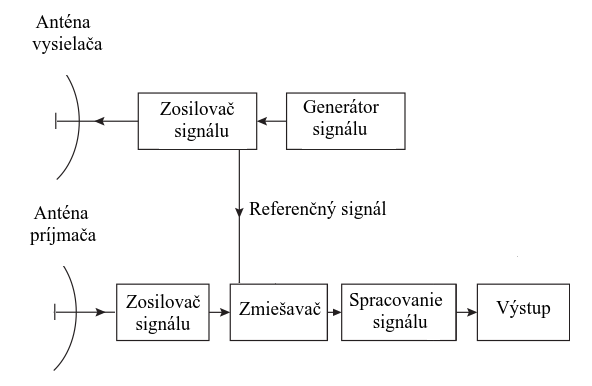
\includegraphics[width=1.0\linewidth]{popis_radaru_own.png}
    \caption{Blokové schéma radaru.}
    \label{fig:popis_radaru_own}
  \end{figure}  
    Radar K-MC4 od Švajčiarskej spoločnosti RFBeam Microwave GmBH sme zvolili ako implicitný radar a budeme to v tejto práci simulovať. Obrázok \ref{fig:popis_radaru_own} znázornuje blokové schéma radaru, ktoré si teraz podrobnejšie rozpíšeme.
    \begin{enumerate}
      \item \textbf{Anténa} je to čo spája radar s vonkajším svetom. Dovoľuje šíriť vysielanú energiu z vysielača, rovnako ako aj zhromažduje zachytenú energiu odrazenú z cieľa.
      \item \textbf{Vysielač} je časť radaru, ktorá generuje a vysiela signál v požadovanej vlnovej dĺžke. 	
      \item \textbf{Príjmač} zachytavá prijatú odrazenú energiu z cieľa. Vzhľadom na vzdialenosť a materiál objektu od ktorého bol signál odrazený sa bude odvíjat jeho intenzita, ktorá dosahuje veľmi malé hodnoty (väčšinou až $10^{-9}$W).
      \item \textbf{Zosilňovač}, v prípade vysielania signálu je jeho úlohou zosíliť signál pred vyslaním, aby sa napriek jeho diaľke, ktorú musí k cieľu uraziť vrátil čo najintenzívnejší. V prípade príjmania signálu ho taktiež zosilňuje, pretože vracajúci sa signál ja veľmi malý.  
      \item \textbf{Zmiešavač} je veľmi dôležitá časť radaru, ktorá nám na výstupe dáva rozdielovú, teda nízku frekvecniu, pre spracovanie prijatého signálu.       
    \end{enumerate}

  \subsection{Dopplerov jav}   
    
    Doplerov jav(efekt) popisuje zmenu vlnovej dlžky príj\-maného signálu voči signálu vysielanému. Čo je spôsobené nenulovou vzájomnou rýchlosťou prímača a vysielača.
    Tento jav nenastáva len pri zvuku, no obecne je pozorovateľný pre ľubovolné elektromagnetické vlnenie. 
    Vlnová dĺžka vysielaná z vlnového zdroja(zvuku, elektromagnetického žiarenia, svetla, atd.) narazí na pohybujúci sa objekt. V závislosti na smere pohybu tohto objektu, sa vlnové dĺžky "stlačia", alebo "rozťiahnu", čo vo výsledku vedie k zmene frekvencie. Odrazený signál so zmenenou frekvenciou sa napríklad pri zvuku prejavý zmeneným tónom pre poslucháča. Teda zmiešaním frekvencie je vo výsledku zmena prechodovej sínusovej frekvencie. Nezáleží či sa pozorovateľ pohybuje k zdroju alebo zdroj k pozorovateľovi\cite{radarsensing}\cite{radarsystems}.
    
    Dopplerova frekvencia sa dá vypočítať ako dvojná\-sobok rozdielu frekvencií ($2 f_{0}$) násobený podielom rýchlosti vozidla ($v$) k rychlosti svetla ($c_{0}$) a kosínusom uhlu pohybu objektu k pozorovateľovi ($\cos \alpha$), znázor\-nené v rovnici \ref{eq:0}.

      \begin{equation} \label{eq:0}
        f_{Dopp} = 2 f_{0} \frac{v}{c_{0}}\cos \alpha
      \end{equation}                

%--------------------------------------------------------
%--------------------------------------------------------
%--------------------------------------------------------
%--------------------------------------------------------
\section{Simuláčné prostredie}

  \subsection{Radar v priestore}

    \hspace{0.6cm}V návrhu simulačného prostredia si pre jednoduchosť vysvetlenia predstavme kocku, ktorá tvorí náš priestor pre umiestnenie radaru, objektu a definovanie podmienok, ktoré pre simuláciu radaru potrebujeme. Ako scénu si predstavme meranie rýchlosti na diaľnici s použitím radaru umiestnenom na vyvýšenou mieste, ktorý sleduje vozidlá na vozovke pod ním.

    V priestore je teda umiestnený radar, pre predstavu napríklad na dialničnom moste, ktorého zorné pole smeruje na diaľnicu pod nim, teda objekty, ktoré radar sleduje ho míňajú po jeho vertikálnej ose, teda prechádzajú pod ním.
    % Táto predstava je základná a postavenia sa budú dať meniť. 

	\begin{figure}[t]
		\centering
		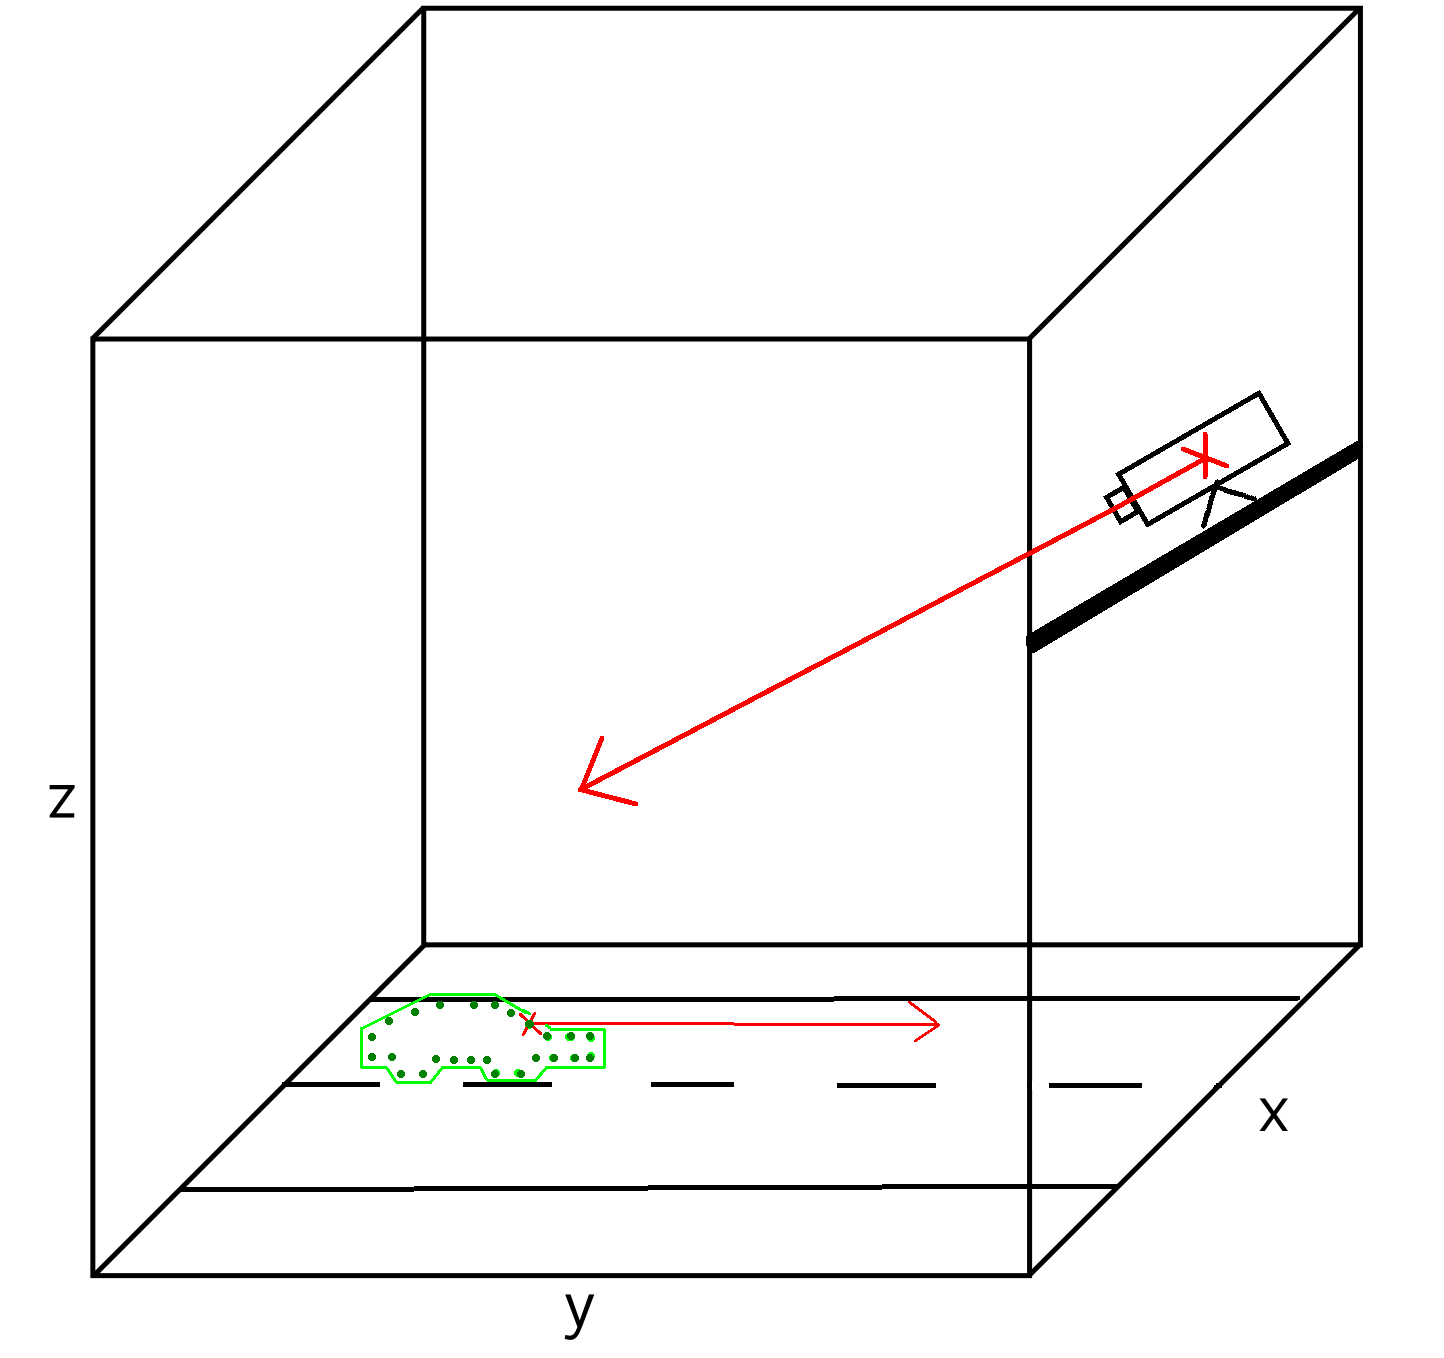
\includegraphics[width=1.0\linewidth]{cube_radar_car.png}
		\caption{Základná predstava priesotru, ktorý budeme simulovať.}
		\label{fig:cube_radar_car}
	\end{figure}

    Radar bude reprezentovaný ako práve jeden nehybný bod v priestore. Tento bod má mať presne určené svoje súradnice v priestore, ktoré charakterizujú jeho polohu. Rovnako obsahuje vektor, ktorý určuje bod kam radar mieri. To znamená, že je nevyhnutne dôležité vedieť kam radar presne mieri počas celej simulácie. Radar bude možné jednoducho natáčať po vertikálnej a horizontálnej ose pomocou jeho vektoru. Voliteľne môžeme pridať aj naklonenie radaru na mieste, do strán, obrázok \ref{fig:cube_radar_car}.
    
    Bod definujúci polohu radaru bude slúžiť ako miesto pre generovanie signálu a zdroj vysielania paprskov na vektor zorného poľa radaru. Podľa súradníc polohy radaru a vektoru radaru sme schopný určiť nevyhnutné uhly a vzdialenosti, ktoré budeme potrebovať pre výpočty simulácie.

  \subsection{Objekt v priestore}
    
    \hspace{0.6cm}Pre správnu funkciu radaru a získanie čo najväčšieho množstva simulačných dát je potrebné rovnako ako aj v návrhu samotného radaru, aj čo najpresnejšie popísať objekt na ktorý budeme v simulácii vysielať naše paprsky, teda cieľ radaru. 

    Objekt preto budeme reprezentovať ako zhluk bo\-dov v určitom tvare, ktorý pripomína objekt reálneho sveta, ako napriklad v našom návrhu, osobné vozidlo.

    Každý tento bod objektu, pričom počet bodov ohraničujúci objekt bude vopred určený, bude pre radar vnímaný ako samostatný objekt a bude obsahovať svoje súradnice v priestore.
    Každý tento bod, sám o seba taktiež objekt bude vykonávať pohyb v priestore, čo bude reprezentovať pohyb celého objektu. Tento pohyb bude reprezentovaný vektorom pohybu bodu, súradnice objektu môžeme pomocou vektoru pohybu odpovedajúcim spôsobom modifikovať.
    %čo je vlastne vektor, ktorý obsahuje aktuálne súradnice bodu vo vzťahu so súradnicami bodu v ďalšom časovom okamžiku . 
    Súčasťou vektoru bude aj rýchlosť pohybu objektu, ktorá bude dopredu definovaná a potrebná pre dalšie výpočty. 
    Všetky body v objekte sa teda budú zdanlivo pohybovať ako jeden celok, znázornené na obrázku \ref{fig:cube_radar_car}.

    Podstatnou charakteristikou bodu bude jeho RCS (Radar Cross-section), ktorý reprezentuje ako intenzív\-ne bude daný bod reagovať na prijatý signál, teda akou silou a smerom odrazi signál näspať. To všetko závisí na simulovanom tvare a materiálu objektu, rovnako ako aj uhlom pod akým je voči paprsku. Táto konštanta nám simuláciu zjednodušuje od jeho fyzíkálnej verzie. RCS sa bude dať jednoducho nastaviť ako vstupná hodnota programu. Rovnako ako súradnice umiestnenia bodov, rýchlosť objektu.

	  \hspace{0.6cm}Radar KMC-4 of spoločnosti RFbeam, ktorý sme sa rozhodli pre túto simuláciu používať ako referenčný má svoje vlastnosti, ktoré musíme implementovať aj do našeho simuláčného radaru. Všetky tieto údaje boli predom získane vyrobcom tohto radaru, firmou RFbeam a sú umiestnené v jeho datasheete \cite{kmc4sheet}, preto ich nemusíme nadobudnúť experimantálne.

  \begin{itemize}
    \item Vysielacia frekvencia radaru KMC-4\\ je 24.150GHz
    \item Zisk antény je 18dB
    \item Zisk vysielača je 13dB
    \item Zisk príjmača je 16dB
  \end{itemize}  

  \section{Charakteristika antény}
    \hspace{0.6cm}Hardwarový modul samotného radaru mieri na určitý bod. Nemôže vysielať a príjmať všetky svoje paprsky do všetkých bodov a smerov rovnomerne. Charakteristika antény, resp. anténový diagram repre\-zentuje aké je potlačenie vysielaného signálu v decibeloch, jednotlivo v horizontálnom a vertikálnom smere vzhľadom na vysielaní signálu od vektoru radaru v uhlových stupňoch. Tento údaj je obsiahnutý v data\-sheete a je len graficky znázornený na obrázku \ref{fig:kmc4_antenna_char}.
	\begin{figure}[t]
		\centering
		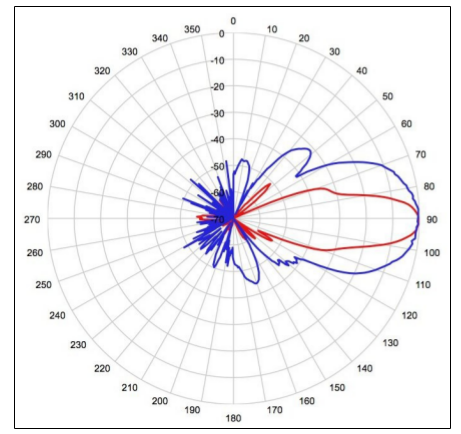
\includegraphics[width=1.0\linewidth]{kmc4_antenna_char.png}
		\caption{Diagram graficky zobrazujúci charakteristiku antény. Ktorý sme použili ako zdroj pre našu textovú verziu charakteristiky antény\cite{kmc4sheet}.}
		\label{fig:kmc4_antenna_char}
	\end{figure}

    Preto je potrebné extrahovať tento útlm antény pre každý stupeň jednotlivo. Pre tento prípad sme použili jednoduchú metódu za pomoci programu Gimp a jeho nástroja pre zmeranie uhlu a to nasledovne. Umiestnili sme jeden koniec pravítka do stredu obrázku a druhý koniec po čiare doprava vedúcej k uhlu 90 stupňov. Tento nástroj ďalej fungoval ako uhlomer a s uhlom v strede obrázku sme pohodlne vyčitali pre každý červený (horizontálny) a modrý (vertikálny) bod jeho útlm v určitom uhle.

    Celý tento proces sa zapisoval do súboru vo formáte .csv. Jeden súbor obsahuje informácie v rozsahu $0^{\circ}-180^{\circ}$, delených po jednom stupni. Pre vertikálny smer a druhý súbor v rovnakom rozsahu pre horizontálny smer.

    Nami získaný (ručne nameraný) počet hodnôt (180) avšak nebude dostačujúci. Nato aby sme signál reken\-štruovali musíme dodržat Nyquistov vzorkovací teorém a predpokladaná frekvencia simulácie bude 10 kHz. To nám spôsobí, že nami získané hodnoty su vo veľmi malom rozsahu a výsledný graf by bol zkockovatelý. Preto musíme tieto hodnoty interpolovať.

    Nami získaný a spracovaný útlm potrebuje pre využitie správny uhol, pre ktorý sa bude určovať. Ten musíme získat v našom trojrozmernom priestore jednotlivo pre horizontálnu a vertikálnu zložku dvojroz\-merného priestoru.

	\begin{figure}[t]
		\centering
		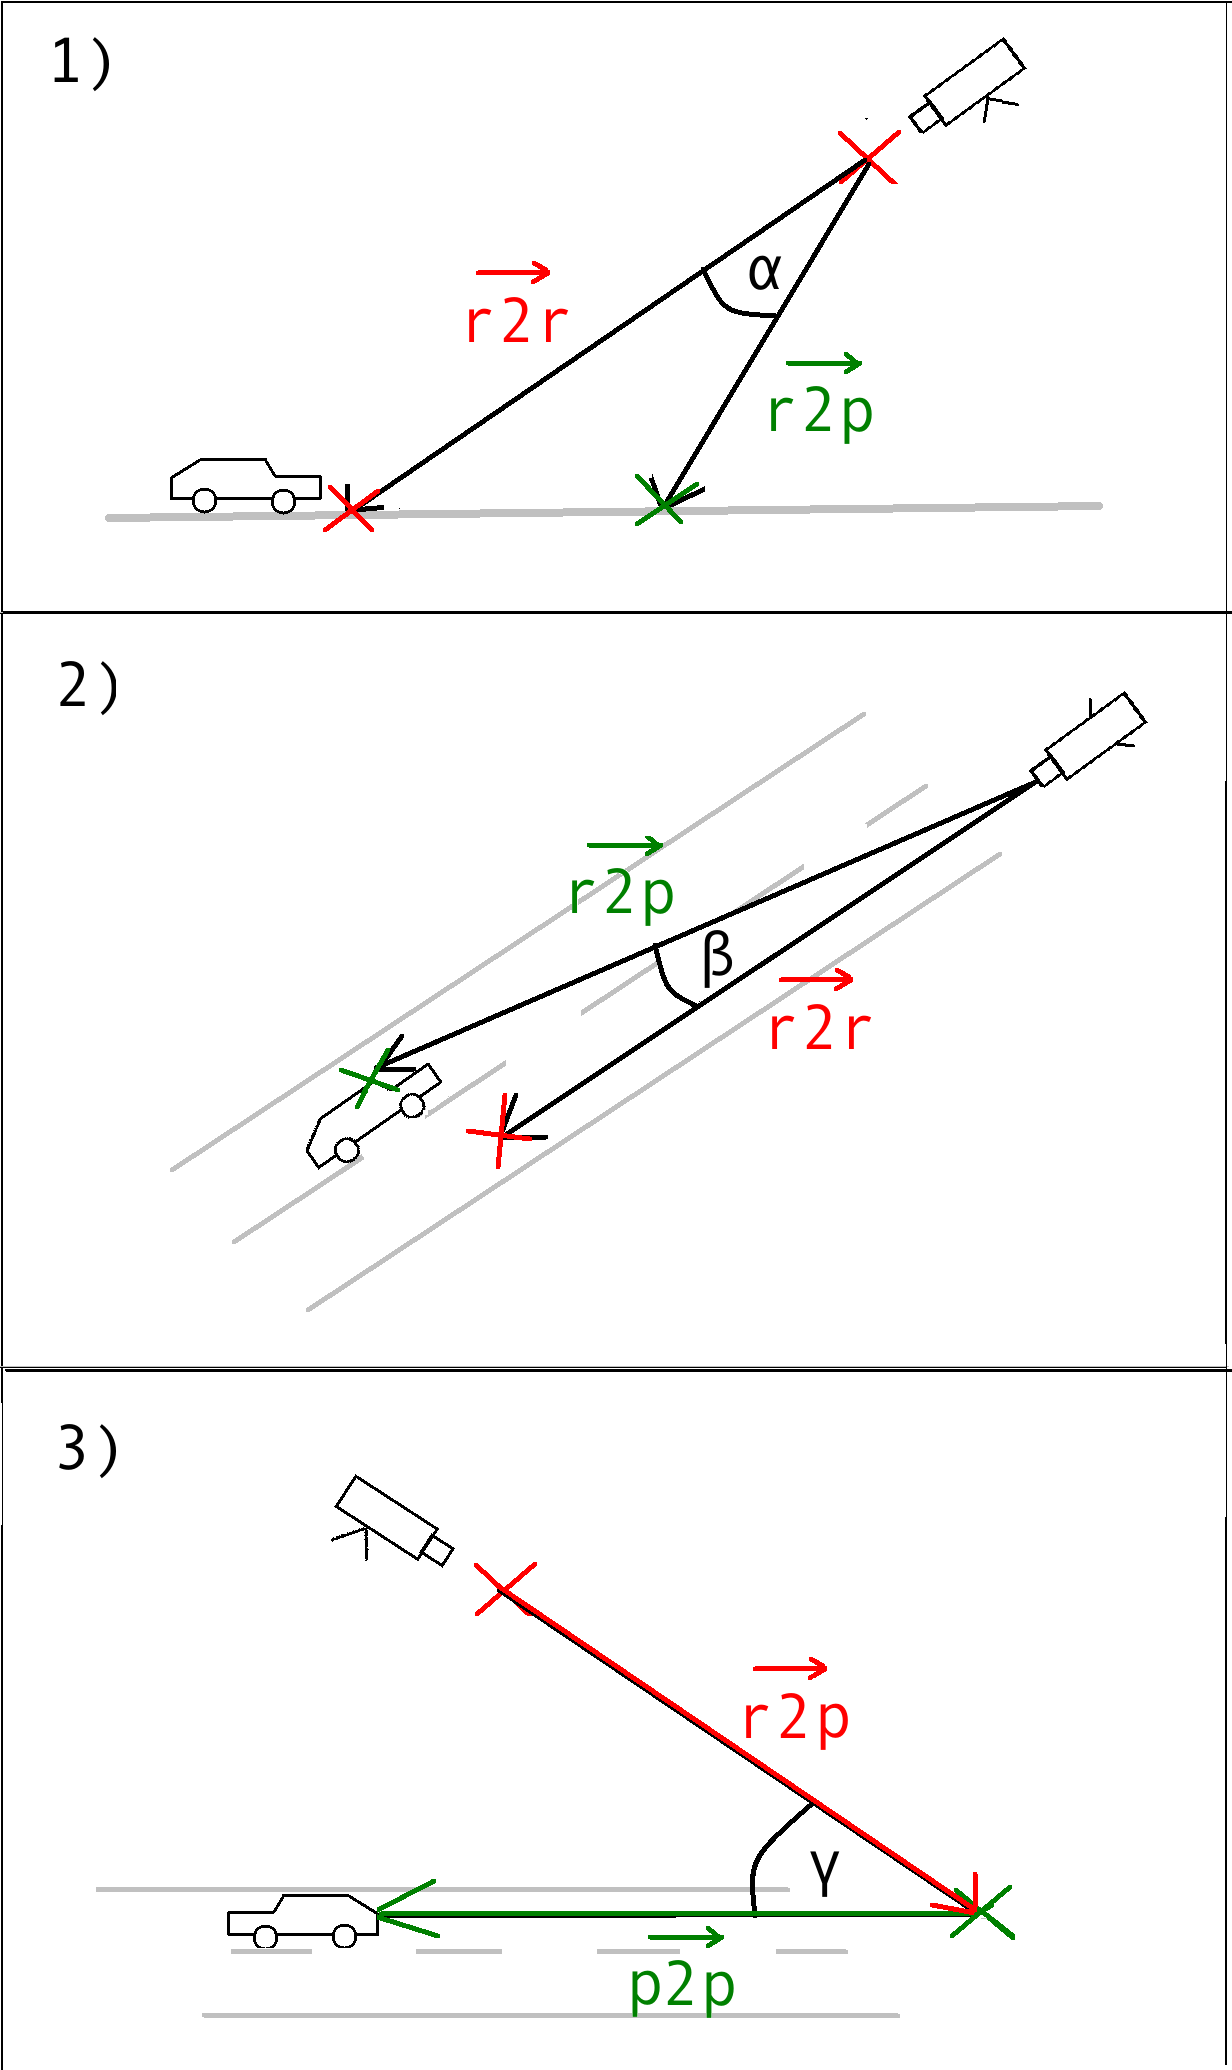
\includegraphics[width=1.0\linewidth]{radar_angles.png}
		\caption{Grafické znázornenie nami riešených a reprezenrtovaných uhlov. 1) Vertikálny 2) Horizontálny 3) Priestorový.}
		\label{fig:radar_angles}
	\end{figure}

    \subsection{Vertikálny uhol}

      Pomocou obrázku \ref{fig:radar_angles} čast 1) vidíme myšlienku pri získavaní hodnoty vertikálneho uhlu. Trojrozmerný priestor si premietnene do dvojrozmerného, teda vyne\-cháme jeho x-ovú zložku.
      Poz\-náme vektor radaru, teda bod v ktorom sa radar nachádza a bod na ktorý mieri, označme si ho ako $\overrightarrow{r2r}$(radar to radar).
      Rovnako poznáme aj aktuálnu pozíciu objektu. Teda vieme určiť vektor od umiestnenia radaru k aktuálnej pozícii objektu v priestore, označme si ho ako $\overrightarrow{r2p}$(radar to point).
      Ziskaný uhol medzi vektormi $\overrightarrow{r2r}$ a $\overrightarrow{r2p}$, je náš žiadúci vertikálny uhol. 

    \subsection{Horizontálny uhol}

    Obdobne ako sme zíkali uhol vertikálny vieme získať aj uhol horizontálny, obrázok \ref{fig:radar_angles} čast 2). V tomto prípade pri premietnutí do dvojrozmerného priestoru vynecháme osu $z$, z trojrozmerného priesotoru.
    Rovnako využijeme vektory $\overrightarrow{r2r}$, $\overrightarrow{r2p}$ a získame požadovaný horizontálny uhol.

    Pre uhlol vertikálny a horizontálny teraz vieme v každom okamžiku simulácie získať uhol radaru voči objektu. Tento uhol použijeme v nami predom pripra\-vených .csv dátach a tým a získame stratu signálu v dB, osobitne pre horizontálny a vertikálny smer v danom časovom okamžiku a usporiadaní objektov priestore. Následne tieto 2 hodnoty vertikálneho a horizontálneho smeru medzi sebou vynásobíme a dostaneme aktuálnu stratu signálu v dB, pre náš bod v priestore voči radaru v danom časovom okamžiku. 
  
  \section{Simulácia útlmu signálu}
    \hspace{0.6cm}Ďalej pracujeme s predstavou nášho priestoru, našej kocky, v ktorej je umiestnený náš radar so svojimi súradnicami rovnako ako aj jeho bod, ktorého pohyb pozoruje. Tieto dva bodi nám tvoria vektor, teda to ako radar mieri na fiktívnu cestu pod ním.

    Z jednej strany kocky na druhú stranu sa nám pohybuje náš objekt, v tomto prípade osobné vozidlo, ktoré je reprezentované zhlukom svojich bodov. Každý bod ma rovnakú rýchlosť a smer pohybu, ktorý určuje jeho vektor pohybu.

    Náš radar virtuálne vysiela nepretržite v každom okamihu pohybu objektu paprsok, čo v našej simulácií znamená veľa výpočtov pre charakteristika tohto imaginárneho paprsku.

    \subsection{Vzdialenosť}

      Vzdialenosť objektu od radaru je potrebné pre výpočet vracajúcej sa energie do radaru, ktorú získame z radar\-ovej rovnice.
      V našom simulačnom prostredí pre získanie hodnoty vzdialenosti využijeme Euklidovu vzdialenosť, čo je metrika daná dvoma vektormi umiestnenými v priestore.
      V našom prípade vektora od bodu radaru k bodu objektu a vektora od bodu objektu k jeho smeru pohybu.

    \subsection{Priestorový uhol}

      \hspace{0.6cm}Pre výpočet frekvencie signálu vracajucého sa späť do radaru budeme potrebovať priestorový uhol, ktorý zviera vektor radaru s vektorom pohybu objektu. Obrá\-zok \ref{fig:radar_angles} časť 3).
      Vektor radaru je nám už dobre známy a máme ho označený ako $\overrightarrow{r2r}$. Vektor pohybu objektu nie je nič iné ako jeho aktuálna pozícia v priestore vo vzťahu s jeho pozíciou v priestore v dalšom časovom okamžiku, označme si ho $\overrightarrow{p2p}$ (point to point).
      Uhol, ktorý tieto 2 vektory zvierajú, je náš požadovaný priesto\-rový uhol.

    \subsection{Prijatý signál}

      \hspace{0.6cm}Po správnom získaní priestorového uhlu, ktorý zviera vektor radaru s verktorom pohybu objektu, sme schopný v každom okamžiku pohybu objektu získať veľkosť sígnalu vracajucého sa od objekt späť do radaru a to pomocou vzťahu:

        \begin{equation} %\label{eq:0}
          F_{r} = 2 * v * \frac{F_{t}}{c} * cos(\gamma)
        \end{equation}   

      Kde rýchlosť objektu $v$ je nami dopredu určená, rovnako ako aj vysielacia frekvencie antény $Ft$ s podie\-lom rýchlosťou svetla $c$. To všetko je v súčine s kosínusom náško priestorového uhlu $\gamma$.
      Celý tento vzťah nie je nič iné ako aplikácia dopplerovho javu.

    \subsection{Radarová rovnica}

      Pre náš finálny výpočet a to kalkuláciu energie, ktorá sa po odraze od objektu do radaru vráti musíme aplikovať nami upravenú radarovú rovnicu \ref{eq:54}.

      \begin{equation} \label{eq:54}
        %P_{r} = \frac{P_{t} * F_{r} * F_{t} * RCS}{(4\pi)^{2} * d^{4} * loss}
        P_{r} = \frac{\lambda * RCS * \sqrt[10]{10^{loss}}}{(4\pi)^{2} * d^{4}}
      \end{equation}   

      \begin{equation} \label{eq:55}
        \lambda = \frac{c}{F_{t}}
      \end{equation}         

      Hodnota $P_{r}$ predstavuje výkon prijatého signálu, ktorý touto rovnicou získame. Vlnová dlžka ($\lambda$) je podiel rýchlosti svetla $c$ s hodnotou frekvencie akú mal vyslaný signál $F_{t}$ z radaru, rovnica \ref{eq:55}. Veličina $RCS$ nám je dobre známa ako Radar cross-section. Hodnota $loss$ predstavuje stratu signálu získanú výpočtami uhlov z charakteristiky antény, na ktorú sme aplikovali logaritmus.
    %$(4\pi)^{2}$
      Hodnota $d$ je vzdialenosť radaru od objektu. Kedže je vysielač aj príjmač umiestnený na spoločnej anténe, umocníme to na štvrtú.

  \section{Simulácia modelovanej scény}
    \hspace{0.6cm}Samotná simulácia je tvorená spojeným všetkých menších celkov, ktoré boli doposiaľ vysvetlnené.

    Celá simulácia sa odvíja od počtu simulačných krokov, ktoré učujú ako podrobne bude každý pohyb objektu spracovaný. Čím viac simulačných krokov, tým podrobnejšie dáta získame, teda tým podrobnejší výsledok zobrazíme. Optimálny počet simulačných krokov našej simmulácie bude $10 000$. Čo bude vo vzťahu s 10 kHz, ktorá je odporúčaná frekvencia simu\-lácie pre splnenie Nyquistovho teorému. V prípade menšieho počtu krokov by mohlo dôjsť k antializasingu. Optimálny ktok simulácie je určený ako podiel počtu simulačných krokov s dráhou akú objekt v simulácií urazí.

    V programe Matlab sa simulácia bodov v našom navrhnutom prostredí vytvára, rovnako ako aj riadi pomocou nástroja HGtransform, ktorý je implicitne obsiahnutý v prostredí Matlab. Tento nástroj spravuje všetky body priestoru, ktoré sme mu vytvorili.\\ S bodmi, ktoré sú na to vopred určené pohybuje v smere v aký sme mu predom definovali. Predpokladáme a určujeme pohyb bodov ako homogenný jav, teda náš pohybujúci objekt nebude zrýchľovat ani spomaľovať.

    V našom trojrozmenrom prostredí nimi môže pohybovať až vo všetkých troch osiach. Nám pre simuláciu vozidla na vozovke bude stačiť práve jedna, ktorá bude charakterizovať jeho pohyb vpred. V budúcnosti pri simulácii objektov pohybujúcich sa vzduchom by sa mohli zísť aj druhá a tretia osa.    

    Jadro simulácie tvorí cyklus, ktorý vykonáva presný počet iterácií, ktorý sa rovná počtu simulačných krokov. V každej jednej iterácii sa pre každý pohybujúci bod jednotlivo určí jeho nová aktuálna pozícia, pričom poznáme aj jeho pozíciu v dalšej iterácií. Tu získame jednoducho tým, že k aktuálnej pozícii pripočítame posun v priestore aký mu určí funkcia HGtransform pre nasledujúci stav. Každému stavu priradzuje stále rovnaký prírastok čo sa javí ako rovnomerný pohyb objektu v priestore. 

    Pre statické body, ako pozíciu radaru v priestore, či bod na ktorý v priestore mieri nám stačí získat práve raz.

    Po získani potrebných pozícií bodov v pristore pre daný okamžik, prebiehajú všetky potrebné výpočty a to:
    \begin{itemize} 
      \item získavanie vzdialenosti
      \item výpočet horizontálneho a vertikálneho uhlov
      \item čo vyústi k výpočtu strát signálu
    \end{itemize}

    Po získaní týchto potrebných medzivýpočtov ich náslende použijeme v rovniciach pre:

    \begin{itemize}
      \item výpočet rozdielu signálu odpovedajúceho \\Dopplerovej frekvencii $F_{r}$ v $Hz$
      \item výpočet výkonu prijatého signálu $P_{r}$ pomocou radarovej rovnice vo $W$
    \end{itemize}

    Výsledkom tohto celého procesu iterácií bude dvojrozmerné pole, ktoré bude obsahovať hodnotu výkonu prijatého signálu. Pre každý jeden bod v jeho každom časovom okamžiku.

    \subsection{Generovanie signálu}

    \hspace{0.6cm}Po skončení tohto sledu iterácií a získaní všetkých potrebných dát a ich naplnení do finálneho poľa výsled\-kov sa spustí ešte jeden identický cyklus s rovnakým počtom iterácií, ktory generuje počiatočný signál v ktorom sa zakompunuje náša prijatá frekvencia $F_{r}$ spolu s výkonom prijatého signálu $P_{r}$.\newline  

    \begin{equation} \label{eq:631}
      \varphi_{d_{t}} = 2\pi * F_{r} * d_{t}
    \end{equation}

    \begin{equation} \label{eq:632}
      result(n) = sqrt(P_{r})*e^{j(\varphi_{1} + \varphi_{d_{t}})}
    \end{equation}

    \begin{equation} \label{eq:633}
    \varphi_{1} = \varphi_{1} +  \varphi_{d_{t}}
    \end{equation}    

    %Výsledný signál z $result(n)$ k záveru preženieme cez Rýchlu Fourierovu transformáciu a pre finálne zobrazenie využijeme spektrum signálu \ref{fig:result}.
    \subsection{Zpracovanie signálu}

    \hspace{0.6cm}V poslednej fáze spracovania signálu nám ostáva už len tento signál segmentovať pomocou Hammingoveho okna cez ktoré tento signal rozdelí na menšie, lepšie spracovateľné časti - rámce. Dĺžka rácma je vypočítaná pomocou primernej hodnoty signálu v da\-nom intervaly, cez funkciu $mean$.

    Tieto rámce ďalej spracuje Rýchla Fourierova transormácia o čo sa postará funkcia matlabu $fftshift$.

    % \begin{equation} \label{eq:xx}
    %     seg = seg - mean(seg);
    % \end{equation} 
    % \begin{equation} \label{eq:xx}        
    %     X = fftshift(fft(seg.*hamming(SEG_LEN)', FFT_LEN));
    % \end{equation} 

\begin{figure}[ht]
\centering
\begin{tabular}{ll}
        ramec = ramec - mean(ramec)
\end{tabular}
\end{figure}

    Tieto rámce ďalej spracuje Rýchla Fourierova transormácia o čo sa postará funkcia matlabu $fftshift$. Symbolický zapísané ako:\newline

% \begin{figure}[ht]
% \centering
% \begin{tabular}{ll}   
\begin{figure}[ht]
\centering
\begin{tabular}{ll}
FazovyPosunFFT ( FFT (\\
   hammingovoOknoPreDanyRamec ) )
\end{tabular}
\end{figure}

        %FFT_posun ( FFT (ramec.hemmingovho_okno(dlzka_ramca)))
        %X = fftshift(fft(seg.*hamming(SEG_LEN)', FFT_LEN));
% \end{tabular}
% \end{figure}



% \begin{figure}[ht]
% \centering
% \begin{tabular}{ll}
%         $seg = seg - mean(seg);$
% \end{tabular}
% \end{figure}
% \begin{figure}[ht]
% \centering
% \begin{tabular}{ll}
%         $X = fftshift(fft(seg.*hamming(SEG_LEN)', FFT_LEN));$
% \end{tabular}
% \end{figure}

    \begin{figure}\centering
      \centering
        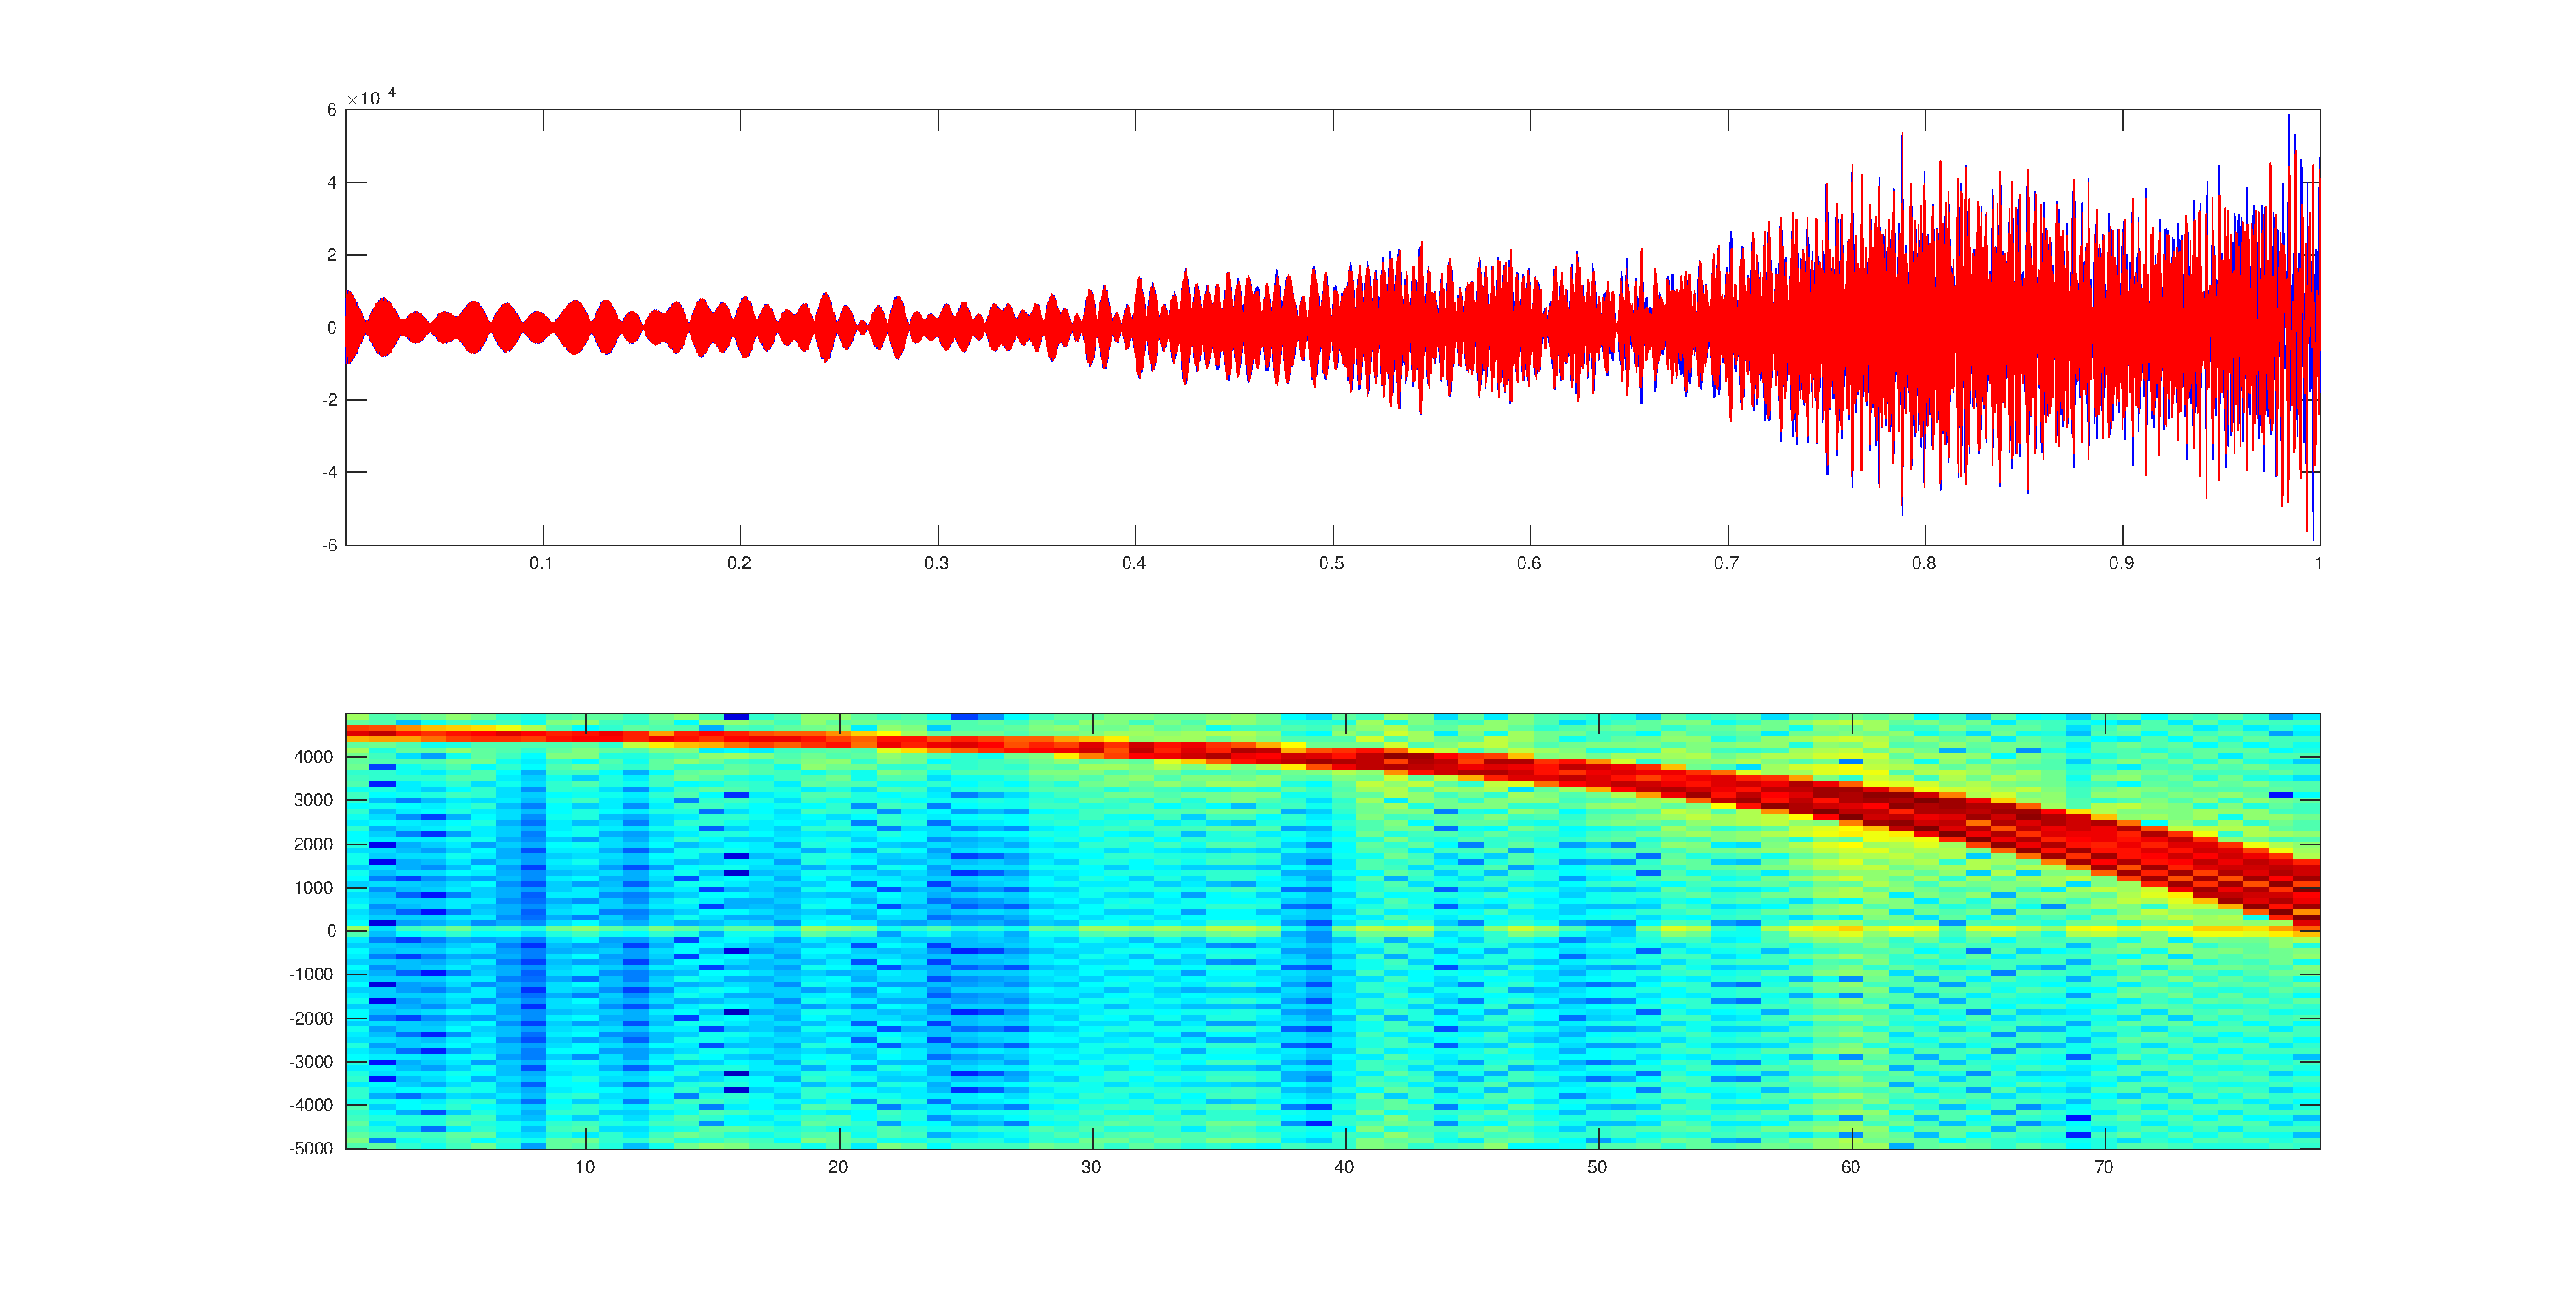
\includegraphics[width=1.0\linewidth,height=2.1in]{output.eps}  
        \caption{Výsledný graf a spektorgram.}
        \label{fig:output}
    \end{figure}        

    Vo výsledku a to na obrázku \ref{fig:output} vidíme výsledok celého procesu spracovania najpr v grafe (horná časť) a následne v spektograme (spodná časť). Vo výslednom grafe je znázornené ako amplitúdy signálu s približujú\-cim sa objektom pomaly stúpajú. Rovnako v spektograme vidíme ako sa znižuje príjmaná frekvencia a názorne aj ako sa delí na viac bodov, ktoré reprezentujú náš objekt.

%--------------------------------------------------------
%--------------------------------------------------------
%--------------------------------------------------------
%--------------------------------------------------------
\section{Záver}
\label{sec:Conclusions}

\hspace{0.6cm}V tejto práci sme sa venovali prezentácií projektu Simulátor širenia radarového signálu. Kde sme si ukázali ako jednoducho a funkčne môžme navrhnúť prostredie spolu s jeho funkčnými časťami pre úspešné simulovanie reaálneho radaru.

Výstupom simulátoru je surový signál odpovedajúci Dopplerovským posunom vznikajúcim v namodelovanom prostredí.

V budúcnosti plánujeme získané dáta z meraní v reálnom prostredí cestnej premávky porovnať s našimi dátami, ktoré budú výsledkom programu po nasimumlované približne rovnakého prostredia. Veríme, že výsled\-ky budú podobné až identické.

\section*{Poďakovanie}
\hspace{0.6cm}Veľmi rád by som poďakoval Ing. Lukášovi Marší\-kovi, ako vedúcemu mojej práce za jeho podporu a cenné rady.
%--------------------------------------------------------
%--------------------------------------------------------
%--------------------------------------------------------
%	REFERENCE LIST
%--------------------------------------------------------
%--------------------------------------------------------
\phantomsection
\bibliographystyle{unsrt}
\bibliography{2017-ExcelFIT-ormos-bib}

%--------------------------------------------------------
%--------------------------------------------------------
%--------------------------------------------------------
\end{document}